%%%%%%%%%%%%%%%%%%%%%%%%%%%%%%

%@天天耶TTY
%试卷模版

\documentclass[11pt,oneside,a4paper,UTF8]{ctexart}

\usepackage{amsmath}    %导入数学包

\usepackage{graphicx}   %导入图片包

\usepackage{placeins}   %隔离figure

\usepackage{float}      %导入浮动体
\usepackage{caption}    %caption为浮动体服务
\usepackage[top=1.5cm,bottom=1.5cm,left=1.5cm,right=1.5cm]{geometry}    %控制页边距

\setlength{\parindent}{0pt}     %全局取消段首缩进

\begin{document}

\zihao{-4} 

\pagestyle{empty}   %把页码去掉

\begin{center}      %这是标题
\zihao{-3}\textbf{这是试卷标题@天天耶TTY}     %小三字号
\end{center}

%%%%%%%%%%以上内容整个copy%%%%%%%%%%

相关内容：这里会写试卷相关内容、有关知识点 \hfill 姓名：\underline{\hspace{2.5cm}}

\vspace*{1\baselineskip}    %空行；1\baselineskip = 正好 1 行的高度
\textbf{零、公式准备}

使用下划线 \_ 输出下标$a_1$、$a_{23}$；

使\^用输出上标$a^1$、$a^{b+c}$；

通过displaystyle使分数线上数字和基本字号一样，使用frac输出分数$\displaystyle\frac{a}{b}$

无displaystyle：$\frac{a}{b}$

使用sqrt输出根号$\sqrt{2}$

使用odot输出圆$\odot O$

使用triangle输出三角形$\triangle ABC$

使用angle输出角$\angle 1$

使用overset+frown输出弧$\overset{\frown}{AB}$

使用circ输出度数$\circ$

使用parallel输出平行$AB\parallel CD$

使用perp输出垂直$AB\perp CD$
\vspace*{1\baselineskip}    %空行；1\baselineskip = 正好 1 行的高度

\textbf{一、选择}

1、这是一道选择题模板，使用dotfill填充点，hspace填充括号空格\dotfill（\hspace{1.5cm}）

A、这是A选项\hfill B、这是B选项\hfill C、@天天耶TTY\hfill D、选项通过hfill均匀铺开

2、这是一道长选项选择题模板，使用tabular表格完成\dotfill（\hspace{1.5cm}）
\begin{tabular*}{\textwidth}{@{}p{0.48\textwidth} p{0.48\textwidth}@{}}     %tabular*{\textwidth} → 表格宽度 = 页面正文宽度；@{} → 去掉左右默认留白
（A）这是选项aaaaaaaaaa； & （B） textwidth → 表格宽度 = 页面正文宽度；\\
（C）@天天耶TTY； & （D） @ → 去掉左右默认留白. 
\end{tabular*}

\textbf{二、填空}

3、这是一道填空题模板，使用underline作为回答区域，hspace控制下划线长度\underline{\hspace{3cm}}.

\textbf{三、解答}

4、这是一道题目在上、图片在下的简答题模板。先书写简答题正文部分。
图片部分使用figure[H]嵌套在figure环境中，H强制放在当前章节。

使用raggedleft右对其；使用raggedright左对其。
使用includegraphics添加图片。

\begin{figure}[H]   %图片嵌套在figure环境中，H强制放在当前章节
\raggedleft     %raggedleft右对其；raggedright左对其
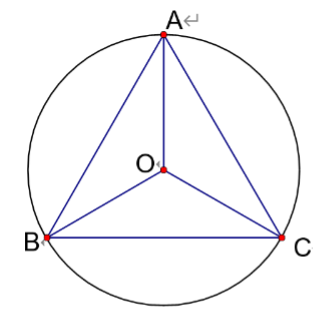
\includegraphics[width=0.2\textwidth]{图片模板.png}  %添加一张当前文本区域宽度0.2的圆图片
\caption{\raggedleft 使用caption添加图片说明。第4题图}
\end{figure}

\newpage    %强制开启新一页  
5、使用newpage强制开启新一页
\vspace*{2\baselineskip}    %空行；2\baselineskip = 正好 2 行的高度

\begin{minipage}{0.7\textwidth}
6、这是一道题目在左边、图片在右边的简答题模板。需要使用minipage进行排版。

需要左边文字内容begin\{minipage\}；右边图片内容begin\{minipage\}。
两个minipage间使用hfill隔开。

注意：minipage不是float环境，图片批注需要使用captionof\{figure\}强行使用。

最后务必使用FloatBarrier隔离后面的figure类。
%当文字过少使用\vspace*{4\baselineskip}空行调整文字和图片的高度关系
\end{minipage}
\hfill
\begin{minipage}{0.28\textwidth}
\raggedleft
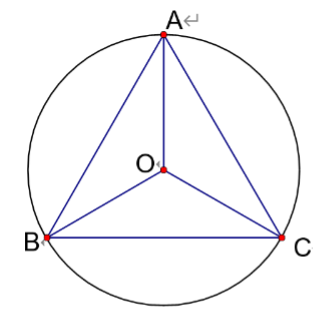
\includegraphics[width=0.8\linewidth]{图片模板.png}
\captionof{figure}{\raggedleft 第6题图}     %在不是浮动体的地方强行使用浮动体
\end{minipage}

\FloatBarrier       %隔离figure

\vspace*{8\baselineskip}    %空行；8\baselineskip = 正好 8 行的高度

\begin{minipage}{0.7\textwidth}
7、当文字过少使用vspace*空行调整文字和图片的高度关系。

注意是在文字的minipage中空行。
\vspace*{6\baselineskip}
\end{minipage}
\hfill
\begin{minipage}{0.28\textwidth}
\raggedleft
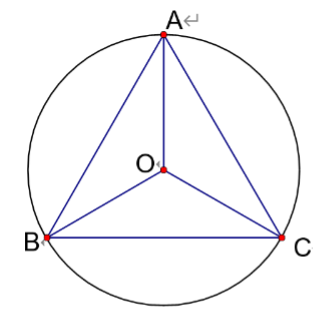
\includegraphics[width=0.8\linewidth]{图片模板.png}
\captionof{figure}{\raggedleft 第7题图}     %在不是浮动体的地方强行使用浮动体
\end{minipage}

\vspace*{6\baselineskip}    %空行；6\baselineskip = 正好 6 行的高度

8、minipage使用完毕后务必使用FloatBarrier隔离后面的figure类，否则会导致图片排版混乱。

\end{document}